\chapter{Validation}
\label{ch:validation}

The calculations were checked against analytic results and against independent numerical methods. This chapter summarises the checks;
the figures and the numbers come from runs of the code with the settings indicated.

\section{Checks against exact results}

\begin{table}[ht]
  \centering\small
  \begin{tabular}{@{}p{7.2cm}p{7.5cm}@{}}
    \toprule \textbf{Check} & \textbf{Result} \\ \midrule
    Slab, single layer, oblique incidence: fraction of particles that interact for $\alpha=90^\circ,\,60^\circ,\,30^\circ$ & $0.5276,\,0.5797,\,0.7771$ against the Beer--Lambert values $0.5276,\,0.5794,\,0.7769$ \\
    Slab, transmission at $\twotheta=0$ for the same orientations & $0.6711,\,0.6287,\,0.4309$ against $0.6714,\,0.6287,\,0.4308$ \\
    Slab, general directions (four cases, both detector sides) & agreement with numerical integration within 0.0005 \\
    Slab, particles entering or leaving through side faces; next interaction of flying particles & brute-force ray stepping: 0 mismatches in 3000 and in 1500 random particles; positions within 0.0003~mm \\
    Cylinder, narrow beam through the axis & $0.7769$ against $1-\e^{-2\mu R}=0.7769$ \\
    Cylinder, beam as wide as the cylinder; beam wider than the cylinder & $0.6716$ against $0.672$; $0.3358$ against $0.336$ \\
    Cylinder, paths from the axis (horizontal, vertical, $45^\circ$, through the axis from an outer layer) & exact \\
    Cylinder, next interaction of random particles, including vertical directions & brute-force ray stepping: 0 mismatches in 1500; positions within 0.0003~mm \\
    Water, $\mu$ of thermal neutrons (Chapter~\ref{ch:builder}) & $5.65$~cm$^{-1}$, the known value is about $5.6$~cm$^{-1}$ \\ \bottomrule
  \end{tabular}
  \caption{Checks against exact results and against brute-force calculations.}
\end{table}

\section{Partially filled layers (version 2.0)}

The tracking was rewritten to include the levels of the material. The checks of Table~\ref{tab:valid-partial} were made; the
script \file{tests/test\_mcams.py} repeats those that do not need the old version.

\begin{table}[H]
  \centering\small
  \begin{tabular}{@{}>{\raggedright\arraybackslash}p{7.2cm}>{\raggedright\arraybackslash}p{7.5cm}@{}}
    \toprule \textbf{Check} & \textbf{Result} \\ \midrule
    Full layers: new code against version 1 with the same random seeds (slab at $90^\circ$, $60^\circ$, $125^\circ$; cylinder) & same particles interact; interaction points, outgoing paths and next interactions equal within $7\times10^{-15}$~mm \\
    Full layers: \code{transmission_vs_angle} and \code{simulate_scattering_orders}, same seeds & identical results (differences $\le 3\times10^{-16}$; identical counts) \\
    Partial layers: outgoing paths for 300 random points and directions, and for the directions $\pm x$, $\pm y$, $z$ & brute-force ray stepping (step $2\times10^{-4}$~mm): agreement within $3\times10^{-4}$~mm, both geometries \\
    Partial layers: next interaction of $2\times10^4$ random particles & optical depth to the new point equal to the random $\tau$ within $10^{-14}$; interaction if and only if $\tau$ is smaller than the optical depth to the exit; all points in material \\
    Slab, uniform beam, fullness $f=0.25,\,0.5,\,0.8,\,1$ & interacting fraction $f\,(1-\e^{-\mu t})$ within the statistical error ($4\times10^5$ particles) \\
    Cylinder, narrow beam through the axis, level inside the beam & $(7/8)(1-\e^{-2\mu R})$: $0.7948$ against $0.7956$ ($\pm0.0006$) \\
    Layer with fill height 0 & identical to a layer with $\mu=0$ \\ \bottomrule
  \end{tabular}
  \caption{Checks of the partially filled layers.}
  \label{tab:valid-partial}
\end{table}

\section{Layers with their own bottom and height (version 2.2)}

The material of a layer is now limited by two planes, $y=b_i$ and $y=t_i$, instead of one. The checks of Table~\ref{tab:valid-band}
were made; those that do not need the old version are in \file{tests/test\_mcams.py} (section~6).

\begin{table}[H]
  \centering\small
  \begin{tabular}{@{}>{\raggedright\arraybackslash}p{7.2cm}>{\raggedright\arraybackslash}p{7.5cm}@{}}
    \toprule \textbf{Check} & \textbf{Result} \\ \midrule
    Version 2.1 against 2.2, the same inputs and random seeds: transmission, scattering counts, transmission by layer, direct factors and mean paths for five samples (full and partially filled slabs and cylinders) & identical: largest difference 0.0 in all 30 quantities \\
    Slab, uniform beam, bands $(b,h) = (-6,5),\,(-2,5),\,(1,6),\,(-6,12),\,(5,3)$~mm in a 10~mm beam & interacting fraction $f\,(1-\e^{-\mu t})$ with $f$ from eq.~(\ref{eq:fullness-general}), within the statistical error \\
    Cylinder, narrow beam through the axis, band from $-1$ to $+3$~mm & $f\,(1-\e^{-2\mu R})$ within the statistical error \\
    \code{height=None}: envelope of the layers; \code{fill_levels}; \code{fill_height} $\equiv$ \code{bottom=y_bottom, height=fill_height} & exact \\
    \code{bottom}/\code{height} together with \code{fill_height} or \code{fullness} & refused with a clear message \\
    Direct method, mean path in a band covering a known part of the beam & $0.75$ of the full value, exact \\ \bottomrule
  \end{tabular}
  \caption{Checks of the layers with their own bottom and height.}
  \label{tab:valid-band}
\end{table}

The comparison with \textsc{pycorrect} (report \emph{pycorrect vs MCAMS}, chapter on partially filled samples) is a further test: the
fullness correction of \textsc{correct}, which is exact for single scattering when the can covers the whole beam and the beam is uniform,
applied to the intensities simulated by \mcams, gives back the true single scattering within 0.2--0.5\% (the statistical error) for
cylinders and flat cells, with the powder at the bottom, in the middle or at the top of the beam.

\section{Disc geometry (version 2.3)}

The disc reuses the path calculation of the slab with a different section, so it was checked both against exact results and
against the slab (Table~\ref{tab:valid-disc}). Section~7 of \file{tests/test\_mcams.py} contains these checks; sections~2 and~3 (paths
against brute-force ray stepping, next interaction) also run on two tilted discs with partially filled layers and bands. The test
script then ran 98 checks.

\begin{table}[H]
  \centering\small
  \begin{tabular}{@{}>{\raggedright\arraybackslash}p{7.2cm}>{\raggedright\arraybackslash}p{7.5cm}@{}}
    \toprule \textbf{Check} & \textbf{Result} \\ \midrule
    Slab and cylinder, version 2.2 against 2.3 (the slab code was reorganised), same inputs and seeds, five samples, 30 quantities & identical: largest difference 0.0 \\
    Outgoing paths in two discs ($\alpha=70^\circ$ and $125^\circ$, partial layers and bands), 300 random points and directions, and along $\pm x$, $\pm y$, $z$ & brute-force ray stepping: agreement within $2\times10^{-4}$~mm (the step) \\
    Next interaction in the same discs, $2\times10^4$ particles & optical depth to the new point equal to the random $\tau$ within $10^{-14}$; interaction if and only if $\tau$ is below the optical depth to the exit; all points in material \\
    Disc of 4000~mm against slab of $4000\times4000$~mm, $\alpha = 60^\circ$, same seeds & identical interaction points; identical outgoing paths for directions that leave through the faces \\
    Thin black disc (20~mm) in a $30\times30$~mm beam, $\alpha=90^\circ$ and $50^\circ$ & hit fraction 0.3486 and 0.2671 against the face area 0.3491 and 0.2674 \\
    Beam inside the disc, $\alpha=90^\circ$ and $60^\circ$ & interacting fraction $1-\e^{-\mu t/\sin\alpha}$ within the statistical error \\
    Disc of 10~mm in a $30\times30$~mm beam, normal incidence & $(\pi R^2/900)(1-\e^{-\mu t})$ within the statistical error \\
    Band from $-6$ to $0$~mm in an 8~mm beam; band larger than the disc & half of the Beer--Lambert value, \code{beam_fullness} 0.5; band cut at the rim \\
    Direct method, normal incidence: $A(0)$ and $A(90^\circ)$ & $A(0)=\e^{-\mu t}$ exactly; $A(90^\circ)$ equal to the separable integral over depth and face (0.21131 against 0.21150, within the error) \\
    Direct method against Monte Carlo, V/Ni/V disc at $\alpha=60^\circ$, three angles & $|z| < 4$ (largest 2.1) \\
    Fraction of a square beam that hits a thin disc, seven beam sizes, three orientations & agreement with \code{face_area_in_beam} within the statistical error (Figure~\ref{fig:discvalid}) \\ \bottomrule
  \end{tabular}
  \caption{Checks of the disc geometry.}
  \label{tab:valid-disc}
\end{table}

\section{Sphere geometry (version 2.4)}

The sphere reuses the segment calculation of the cylinder with spherical surfaces. Section~8 of \file{tests/test\_mcams.py} contains
the checks of Table~\ref{tab:valid-sphere}; sections~2 and~3 also run on two spheres, one with a partially filled layer and one with
bands. The test script now runs 124 checks.

\begin{table}[H]
  \centering\small
  \begin{tabular}{@{}>{\raggedright\arraybackslash}p{7.2cm}>{\raggedright\arraybackslash}p{7.5cm}@{}}
    \toprule \textbf{Check} & \textbf{Result} \\ \midrule
    Slab, disc and cylinder, version 2.3 against 2.4 (the cylinder code was reorganised), same inputs and seeds, 30 quantities & identical: largest difference 0.0 \\
    Outgoing paths in the two spheres, 300 random points and directions, and along $\pm x$, $\pm y$, $z$ & brute-force ray stepping: agreement within $4\times10^{-4}$~mm (twice the step) \\
    Next interaction in the same spheres, $2\times10^4$ particles & optical depth to the new point equal to the random $\tau$ within $10^{-14}$; interaction if and only if $\tau$ is below the optical depth to the exit; all points in material \\
    Points and directions rotated together by a random rotation (three full layers) & paths unchanged within $10^{-13}$~mm \\
    Pencil beam through the centre, $R=5$~mm, $\mu=0.2$~mm$^{-1}$ & $1-\e^{-2\mu R}$: 0.8636 against 0.8647 (within the error) \\
    Beam larger than the sphere ($12\times12$~mm) & $\frac{2\pi}{w_bh_b}\int_0^R(1-\e^{-2\mu u})\,u\,\deriv u$: 0.3834 against 0.3834 \\
    Black sphere in an $8\times8$~mm beam & hit fraction 0.9722 against \code{section_area_in_beam} 0.9717; $\pi R^2$ for a wide beam \\
    Half-filled sphere (up to $y=0$), vertical line beam & $\frac18\int_{-4}^{0}(1-\e^{-2\mu\sqrt{R^2-y^2}})\,\deriv y$: 0.4101 against 0.4115 (within the error); fullness 0.5 \\
    Direct method, $A(0)$ and mean path, beam larger than the sphere & $A(0) = \int L\e^{-\mu L}\deriv A/\int L\,\deriv A$: 0.24248 against 0.24249; mean path $\tfrac43\pi R^3/(w_bh_b)$ within the error \\
    Direct method against Monte Carlo, Ni sphere in a V shell, three angles & $|z|<4$ (largest 0.9) \\
    Factory: radii, vertical extent & \code{make_sample("sphere", ...)}: radii and $\pm R_\mathrm{out}$ as expected \\ \bottomrule
  \end{tabular}
  \caption{Checks of the sphere geometry.}
  \label{tab:valid-sphere}
\end{table}

\section{Worked examples in the notation of CORRECT (manual 2.5)}

Each example of Chapter~\ref{ch:correct} ends with a closure test: the simulated intensities of the three runs, corrected with the six
attenuation factors of the direct method and the simulated multiple scattering, give back the true unattenuated scattering of sample,
container and heater. For the five geometries the sample is recovered within 0.1--0.4\% (1--3 standard errors), and the container and
heater within their statistical errors (1--2\%). Some exact values are also reproduced: for a plate at $\twotheta=0$ all the factors of
a run equal $\e^{-\sum\mu_k t_k}$ (0.6787, 0.9728, 0.9909 in Example~15, and 0.6393 for the tilted disc of Example~16).

\section{All the factors and the least-squares correction (manual 2.6)}

In Example~18 the least-squares correction with the runs sch, ch, h reproduces the Paalman \& Pings chain to $6\times10^{-16}$; with four
other sets of runs (sc, c; sh, h; s; all seven) the sample is recovered within 0.1--0.4\% and $\chi^2$ is compatible with the number of
degrees of freedom. The diagnostic factors reproduce exact values ($A_{s,h} = \e^{-0.0459\times0.2} = 0.9909$ for the heater crossed
twice). A high-statistics run of the empty can ($2\times10^7$ particles) agrees with the direct method within $0.05\% \pm 0.19\%$.

\section{Consistency between the methods}

\begin{itemize}
  \item With all scatter fractions equal to 1, the \emph{single} transmission by layer of Chapter~\ref{ch:lastlayer}, averaged over the layers, reproduces the transmission of
        Chapter~\ref{ch:transmission} to rounding ($2\times10^{-15}$), for both geometries; the per-layer vectors agree with a direct calculation from the first
        interaction points to $3\times10^{-15}$.
  \item The particle-by-particle counts (Chapter~\ref{ch:scattering}) and the exact-direction estimate (Chapter~\ref{ch:lastlayer}) are two independent ways of
        computing the same quantity. Figure~\ref{fig:valid}(b) compares them for a tall two-layer cylinder with absorption, in a $\pm5^\circ$ azimuth window:
        they agree within the statistical error, for single and for multiple scattering.
  \item The bookkeeping closes: incident = no interaction + absorbed + exited (+ unfinished = 0), with and without absorption.
\end{itemize}

\begin{figure}[ht]
  \centering
  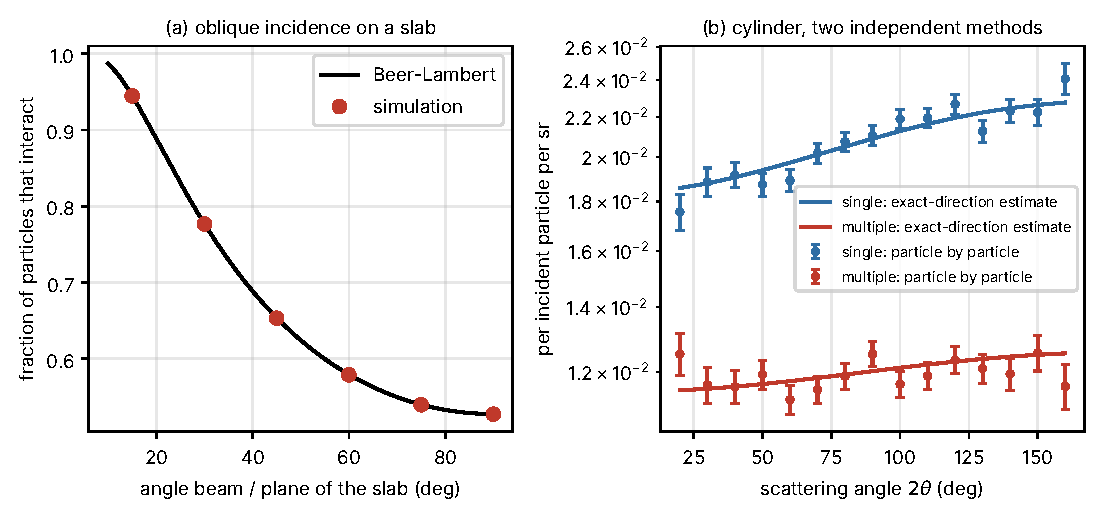
\includegraphics[width=\textwidth]{fig_validation}
  \caption{(a)~Fraction of particles that interact in a very wide single-layer slab ($\mu=0.25$~mm$^{-1}$, thickness 3~mm) versus the angle
  between the beam and the plane of the slab: simulation and Beer--Lambert law. (b)~Cylinder with absorption: single and multiple scattering per
  steradian, particle-by-particle counts (points with Poisson error bars) and exact-direction estimate (lines).}
  \label{fig:valid}
\end{figure}

\section{Formula reader and layer builder}

About twenty formulas were read correctly, including nested parentheses, hydrates, fractional amounts, isotopes and the shorthands D and T
(\code{Dy} is read as dysprosium and \code{Ti} as titanium, not as D or T followed by a letter); twelve incorrect formulas are rejected with a message. The
molar mass, the proportionality of $\mu$ with the density, the equality of per-atom and per-formula-unit inputs, the user overrides and the error messages were tested.

\section{Direct method (version 2.1)}

The direct method of Chapter~\ref{ch:direct} was checked against analytic results (slab in transmission and reflection, also partially
filled), against exact one-dimensional integrals (cylinder with a container and a narrow beam at $0^\circ$ and $180^\circ$) and against a converged
deterministic grid (furnace factors at $30^\circ$ and $150^\circ$): all within the statistical error (Table~\ref{tab:direct-exact}). It agrees with
the Monte Carlo within the statistics for slabs, tilted slabs, cylinders, partially filled containers and non-uniform beams
(Table~\ref{tab:direct-mc}), and its single-scattering intensity reproduces the single-scattering counts of the particle-by-particle simulation
($\chi^2$ per bin 0.67, Figure~\ref{fig:direct-orders}). The same checks, in a shorter form, are part of \file{tests/test\_mcams.py}.

\section{What has not been validated}

The adapter to the package \code{periodictable} has been tested only against a stand-in object with the same attributes (it was not installed in the
environment where the package was developed), so it should be checked on your system (Chapter~\ref{ch:builder}). No comparison with measured data has been made:
the example layers are illustrative.
